\subsection{Fitting the Chambers formula to the data}
The Boltzmann transport model is way more complex than the Drude model, and can have a non-convex
optimization landscape. So we used a more sophisticated global optimization algorithm, called
differential evolution. This is a similar to a genetic algorithm, but with a few differences. It
works by creating a population of candidate solutions, and then iteratively improving them by
combining the best solutions.

The tight-binding model for the Fermi surface of LSCO has already been studied by others, so we
just used the parameters from the literature. The adjustable parameters are the scattering model
parameters and the energy scale, which is a scaling factor for the tight binding parameters,
defined as the value of $t$. The other tight binding parameters ($t'$, $t''$, and $t_z$) are
defined as multiples of $t$.

\begin{figure}
    \centering
    \begin{subfigure}{0.48\textwidth}
        \centering
        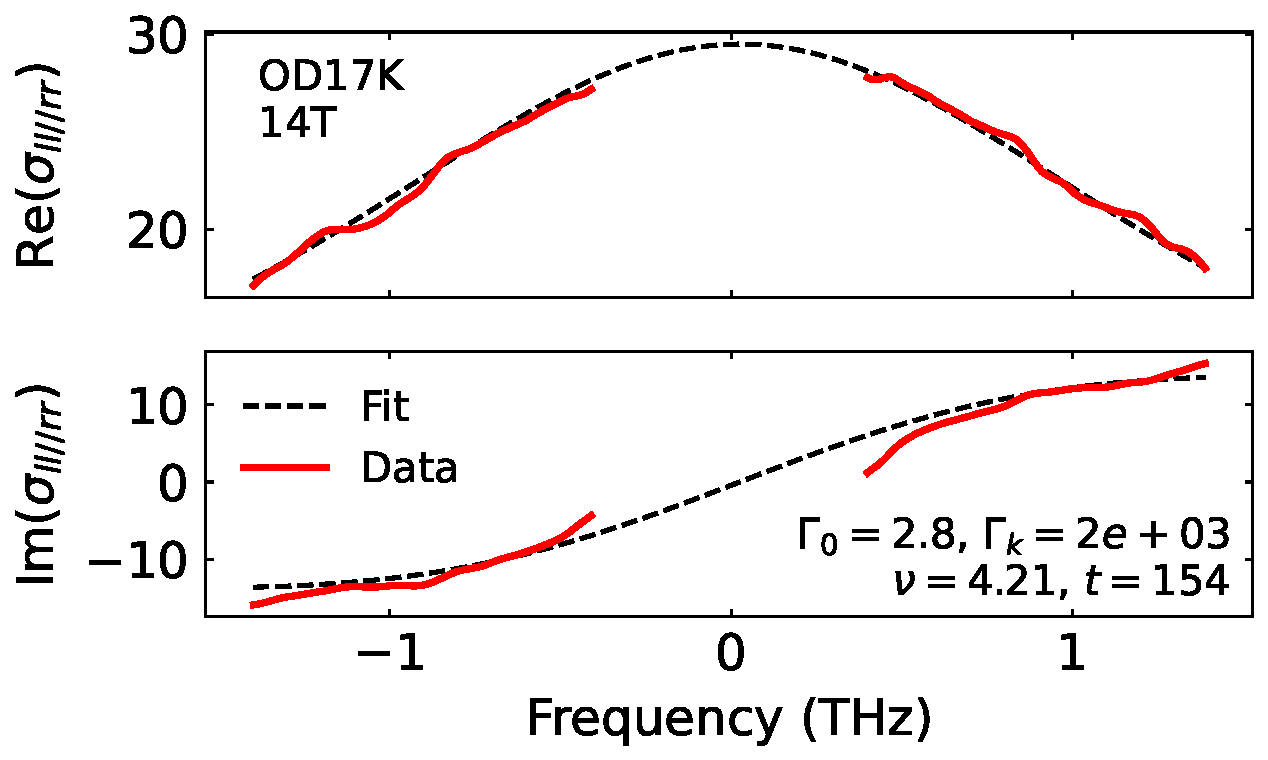
\includegraphics[width=\textwidth]{figures/fit_example_complex}
        \caption{Full complex fit}
    \end{subfigure}
    \begin{subfigure}{0.48\textwidth}
        \centering
        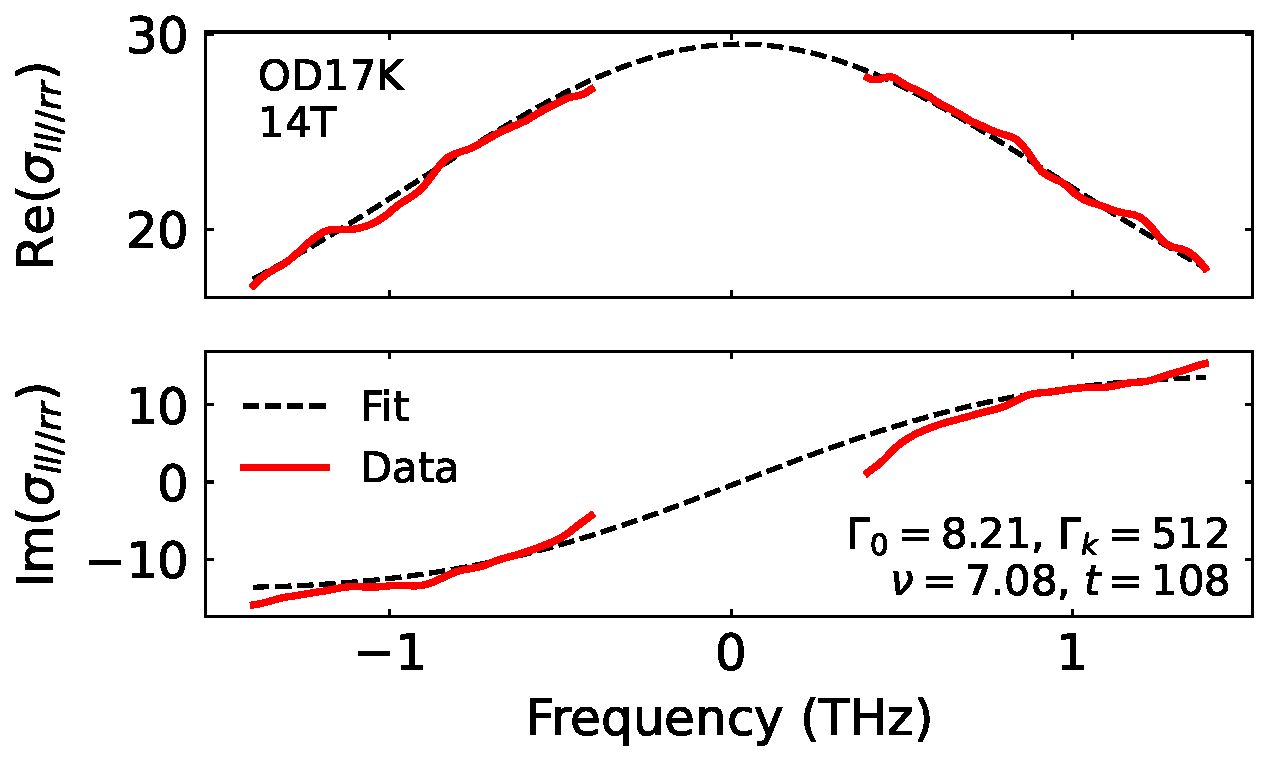
\includegraphics[width=\textwidth]{figures/fit_example_real}
        \caption{Real part fit}
    \end{subfigure}
    \caption{An example of a fit to the data. (a) shows a fit using the full conductivity data,
        while (b) shows a fit using only the real part of the conductivity. As you can see, both
        approaches do a fine job of fitting the data. Another thing to note in these plots is the
        large error and noise, especially in the imaginary part of the conductivity. The ``wrong''
        curving direction in low frequencies in the imaginary part is only present in some of the
        data, and the source is not physical.}
    \label{fig:fitting_example}
\end{figure}

Since the data is noisy and does not exhibit complex behavior, the fitting optimization problem is
very challenging. We have data for different doping levels and different magnetic fields, so a
naïve approach would be to fit the data for each doping level and each magnetic field separately.
However, fitting only to one curve at a time would not constrain the parameters enough and would
lead to many different combinations of parameters fitting the data well. So, we fit multiple
magnetic fields for each doping level simultaneously to constrain the parameters better. To make
sure our fit makes sense, we redo the fit for different sets of magnetic fields and compare the
fitting parameters. If they are consistent, we can be confident in the results.

Even with all that, the problem of an ill-posed optimization problem remains. By carefully
inspecting the fitting tendencies, we found out that this is due to the fact that the imaginary
part of the measured optical conductivity has large errors. This causes the fitting algorithm to
try to ``kill'' any features in the curve, which leads to arbitrarily large values for the
anisotropic scattering parameters. To mitigate this, we only fitted the real part of the optical
conductivity. Doing this, we can see that eventhough we have ignored the imaginary part, it will
also be fitted well, without exploding the fit parameters. This is similar to what we believe
Legros et al.\cite{legros2022} did for their own fits.

\begin{figure}
    \centering
    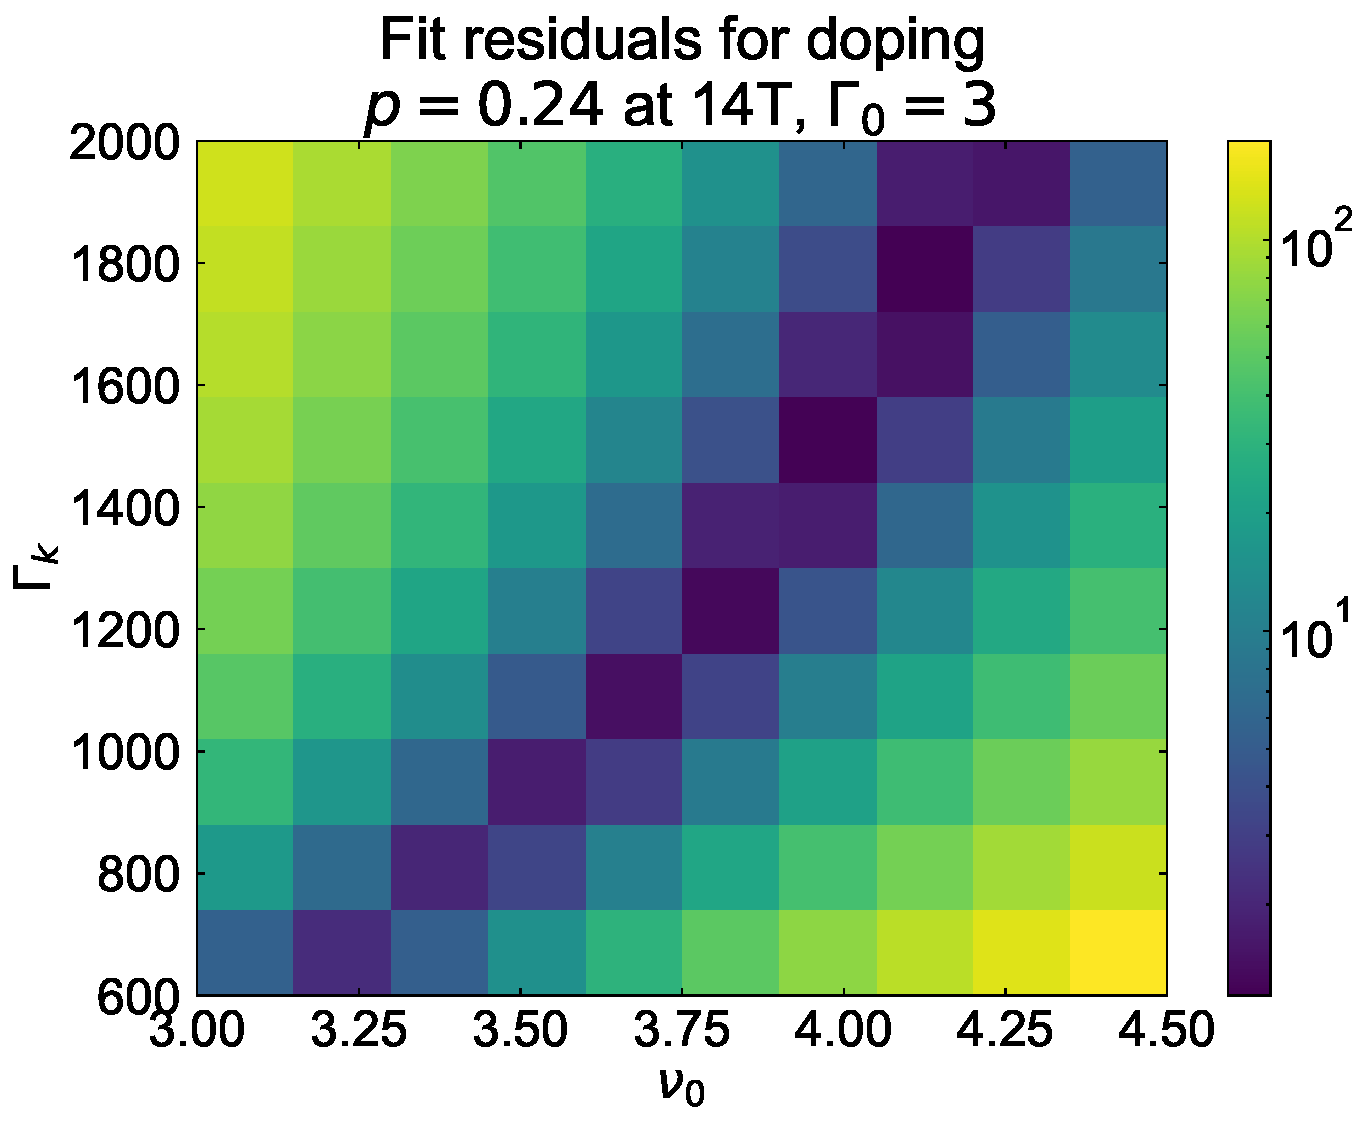
\includegraphics[width=0.5\textwidth]{figures/residuals_degenerate}
    \caption{The extremely degenerate nature of the fitting problem. This plot shows how many pairs
        of values for $\Gamma_k$ and $\nu$ make a good fit for the data.}
    \label{fig:residuals_degenerate}
\end{figure}
